% -----------------------------------------------------------------------------
% Closing slide.  Deliberately outside the section machinery: no breadcrumb, no
% entry in the lecture map, no frame number.  The accent along the bottom is the
% signature of the whole talk -- a flat, nearly symmetric profile that breaks
% into a single peak, which is where the head forms.
% -----------------------------------------------------------------------------
\begin{frame}[plain,noframenumbering]
  \begin{tikzpicture}[remember picture,overlay]

    \fill[HydraNavy] (current page.south west) rectangle (current page.north east);

    \node[anchor=center,inner sep=0pt] at ([xshift=2.35cm]current page.center)
      {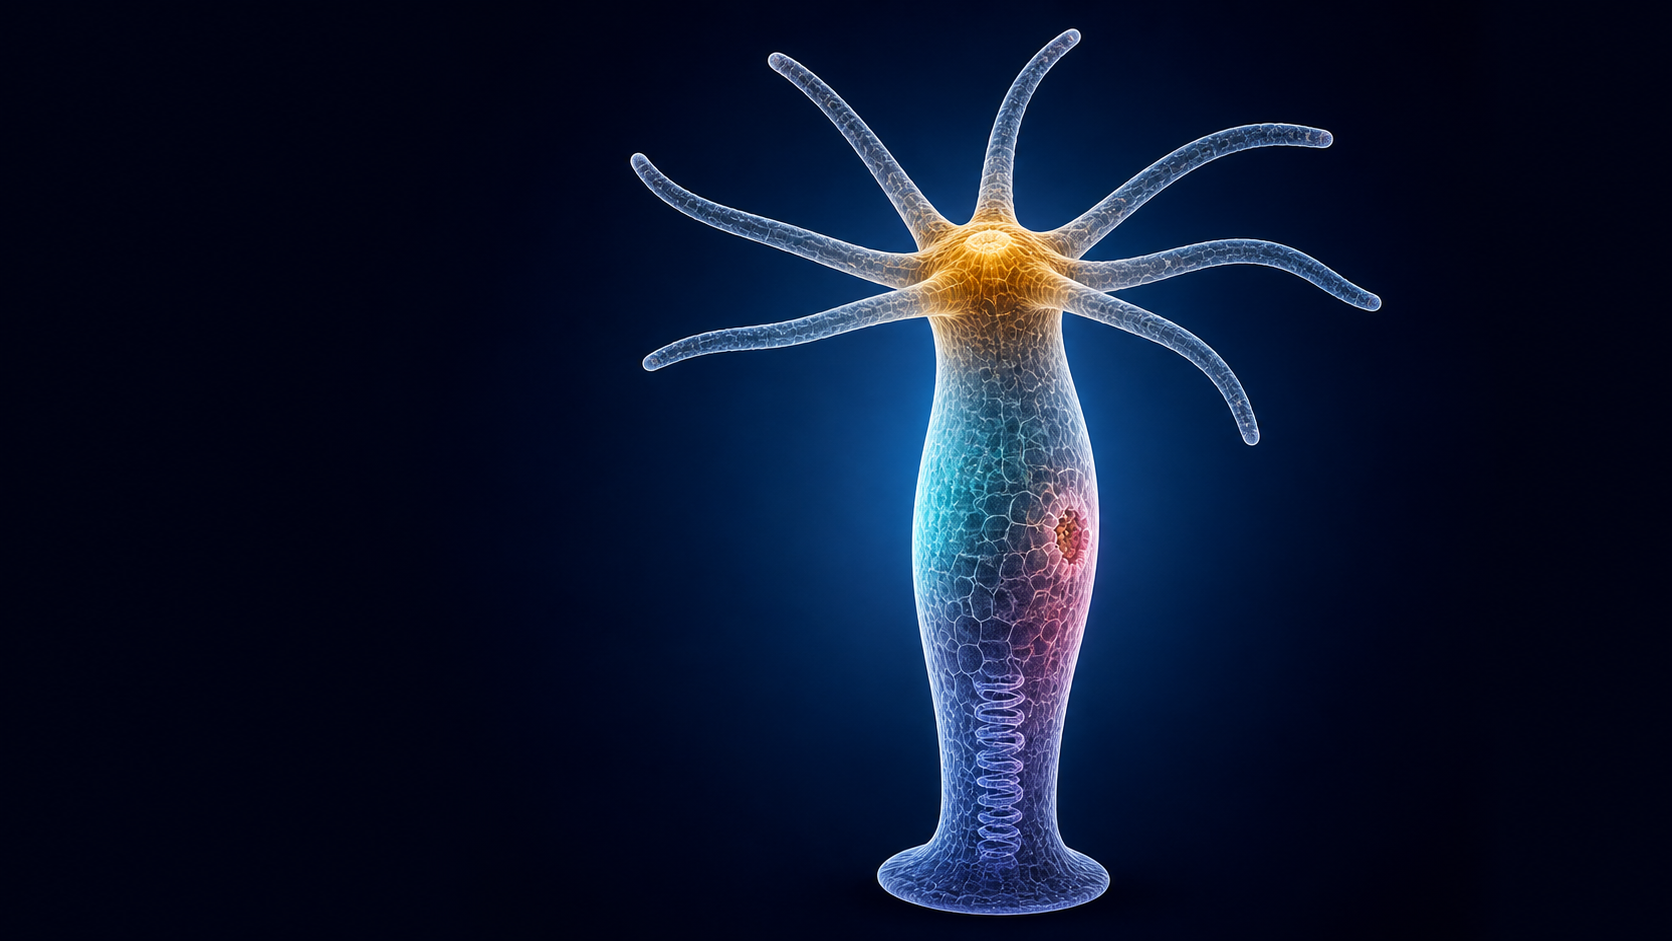
\includegraphics[width=1.34\paperwidth,height=1.34\paperheight,
        keepaspectratio]{figures/common/hydra_zoom_map.png}};

    \fill[HydraNavy,opacity=.97]
      (current page.south west)
      rectangle ([xshift=8.30cm]current page.north west);
    \fill[HydraNavy,opacity=.30]
      ([xshift=8.30cm]current page.south west)
      rectangle (current page.north east);

    % --- heading -----------------------------------------------------------
    \fill[HydraGold]
      ([xshift=0.86cm,yshift=-1.15cm]current page.north west)
      rectangle ++(0.90cm,0.055cm);

    \node[anchor=north west,text=HydraWhite,
      font=\bfseries\fontsize{34}{38}\selectfont]
      at ([xshift=0.82cm,yshift=-1.72cm]current page.north west)
      {Thank you};

    \node[anchor=north west,text=HydraCyan,
      font=\fontsize{14}{18}\selectfont]
      at ([xshift=0.86cm,yshift=-3.30cm]current page.north west)
      {for your attention};

    \draw[HydraLine,line width=0.6pt]
      ([xshift=0.86cm,yshift=-4.15cm]current page.north west)
      -- ++(6.30cm,0);

    % \node[anchor=north west,text=HydraBody,text width=6.30cm,align=left,
    %   font=\fontsize{8.6}{11.6}\selectfont]
    %   at ([xshift=0.86cm,yshift=-4.50cm]current page.north west)
    %   {\hyphenpenalty=10000\exhyphenpenalty=10000\relax
    %    From a nearly symmetric sphere to a single head: local activation,
    %    long-range inhibition, and one unstable mode -- supplied either by a
    %    second morphogen or by the mechanics of the tissue itself.};

    % --- accent: symmetry breaking into one organizer -----------------------
    % \begin{scope}[shift={([xshift=0.88cm,yshift=0.92cm]current page.south west)}]
    %   \draw[HydraLine,line width=0.5pt] (0,0) -- (6.26,0);
    %   \draw[HydraGold,line width=1.25pt,smooth,samples=140,domain=0:6.26]
    %     plot (\x,{1.02*exp(-((\x-2.30)*(\x-2.30))/0.34)});
    %   \fill[HydraGold] (2.30,1.02) circle[radius=0.070cm];
    %   \node[anchor=west,text=HydraMuted,
    %     font=\fontsize{6.4}{7.6}\selectfont]
    %     at (3.30,0.62) {one head, here};
    % \end{scope}

    % \node[anchor=south west,text=HydraMuted,
    %   font=\fontsize{7.4}{9}\selectfont]
    %   at ([xshift=0.88cm,yshift=0.42cm]current page.south west)
    %   {\insertauthor};

  \end{tikzpicture}
\end{frame}
